% Compile with: xelatex helgarfri_cv_en.tex
% For exact website look, install Fira Code and use: \setmainfont{Fira Code}

\documentclass[11pt,a4paper]{article}

\usepackage[utf8]{inputenc}
\usepackage[T1]{fontenc}
\usepackage{fontspec}
\usepackage{geometry}
\usepackage{xcolor}
\usepackage{hyperref}
\usepackage{fontawesome5}
\usepackage{tcolorbox}
\usepackage{tikz}
\usepackage{enumitem}
\usepackage{ragged2e}
\usepackage{graphicx}
\usepackage{paracol}
\usepackage{eso-pic}

\geometry{a4paper, left=0pt, top=0pt, right=0.5in, bottom=0.5in}
\newlength{\sidebarwidth}
\AddToShipoutPictureBG{\AtPageLowerLeft{\textcolor{sidebar}{\rule{\sidebarwidth}{\paperheight}}}}
\newlength{\photoheight}
\setlength{\photoheight}{236pt}
\AddToShipoutPictureBG*{\AtPageUpperLeft{\raisebox{-\photoheight}{\begin{tikzpicture}[x=1pt, y=1pt]
  \useasboundingbox (0,0) rectangle (\sidebarwidth, \photoheight);
  \path[clip] (0, \photoheight) -- (\sidebarwidth, \photoheight) -- (\sidebarwidth, 0) -- (0, 51) -- cycle;
  \node[anchor=south west, inner sep=0, outer sep=0] at (0,0) {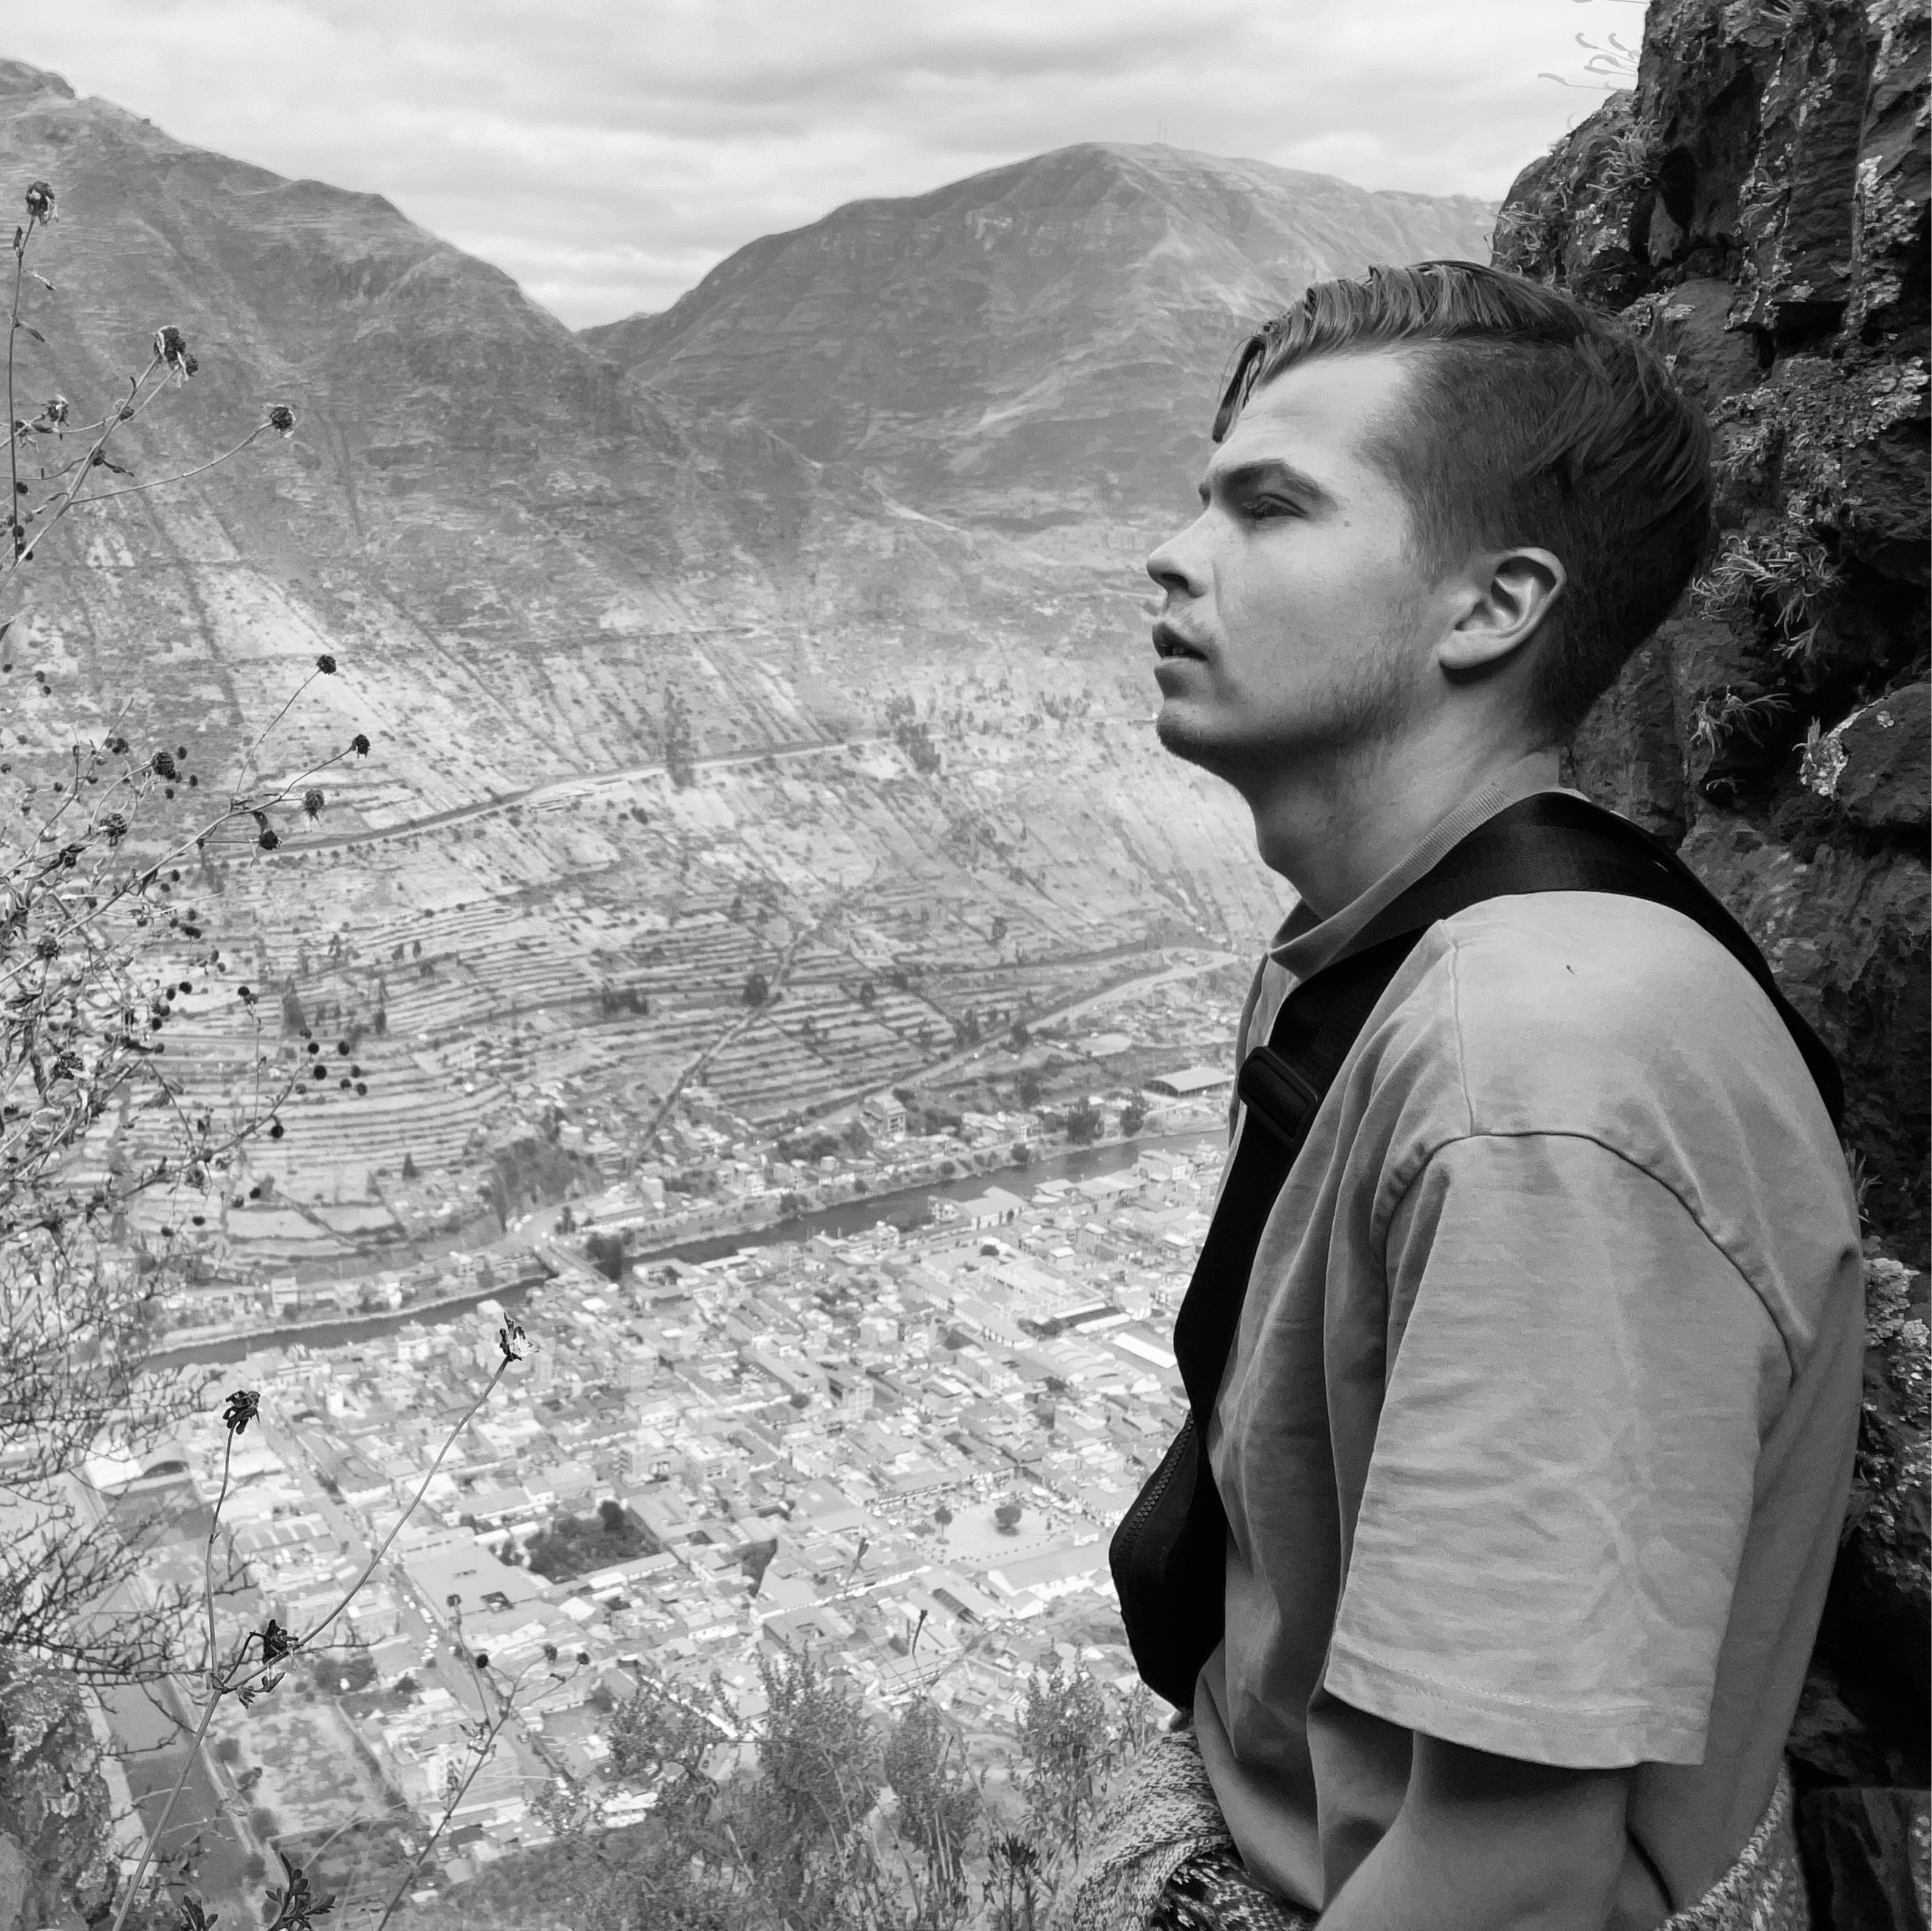
\includegraphics[width=\sidebarwidth, keepaspectratio=true]{helgarfri-cropped.jpg}};
\end{tikzpicture}}}}
\setmonofont{DejaVu Sans Mono}[Scale=0.92]
\renewcommand{\familydefault}{\ttdefault}

\pagestyle{empty}
\RaggedRight
\linespread{1.3}\selectfont

\definecolor{textcolor}{HTML}{1a1a1a}
\definecolor{boxbg}{HTML}{fafafa}
\definecolor{boxborder}{HTML}{e8e8e8}
\definecolor{linkcolor}{HTML}{1a1a1a}
\definecolor{sidebar}{HTML}{242424}
\definecolor{sidebartext}{HTML}{e8e8e8}
\definecolor{sidebarhead}{HTML}{cccccc}

\hypersetup{colorlinks=true, urlcolor=linkcolor, linkcolor=linkcolor}

\newcommand{\sidebarhead}[1]{%
  \textcolor{sidebarhead}{\textbf{\small #1}}\\[0.35em]%
}

\newcommand{\rightsection}[1]{%
  \vspace{1.5em}%
  \noindent\textcolor{textcolor}{\textbf{\large #1}}\\[0.4em]%
  \noindent\rule{0.25\textwidth}{0.35pt}\\[0.55em]%
}

\begin{document}
\setlength{\sidebarwidth}{0.41\textwidth}
\addtolength{\textheight}{22pt}

\vspace*{0pt}%
\noindent
\setcolumnwidth{0.41\textwidth, 0.56\textwidth}
\setlength{\columnsep}{0pt}
\begin{paracol}{2}

  \parbox[t]{\linewidth}{%
    \parindent=0pt
    \color{sidebartext}\small\raggedright
    \setlength{\baselineskip}{1.12\baselineskip}%
  \rule{0pt}{\photoheight}%
  \vspace{0.22em}%
  \leftskip=30pt \rightskip=30pt

  \sidebarhead{brief intro}
  i'm a developer and aspiring computer scientist, with a focus on web development.
  i have experience building a full web stack from the ground up with express.js and postgresql.
  i enjoy solving problems and want to work on challenging projects in data engineering, software development, or analytics.
  \vspace{1.2em}

  \sidebarhead{contact}
  \faPhone\ +354 837 8222\\[0.25em]
  \faEnvelope\ \href{mailto:helgi@helgarfri.is}{\textcolor{sidebartext}{helgi@helgarfri.is}}\\[0.25em]
  \faGithub\ \href{https://github.com/helgarfri}{\textcolor{sidebartext}{helgarfri}}\\[0.25em]
  \faGlobe\ \href{https://helgarfri.is}{\textcolor{sidebartext}{helgarfri.is}}\\[0.25em]
  \faMapMarker*\ ólafsgeisli 89, 113 reykjavík
  \vspace{1.2em}

  \sidebarhead{skills}
  \begin{itemize}[left=3.2em, nosep, itemsep=0.22em]
    \item javascript / typescript
    \item node.js / express
    \item postgresql
    \item git / github
    \item react.js / next.js, html / css
  \end{itemize}
  \vspace{0.85em}

  \sidebarhead{languages}
  \begin{itemize}[left=3.2em, nosep, itemsep=0.28em]
    \item icelandic — native
    \item english — fluent
    \item spanish — intermediate
  \end{itemize}
  }%

\switchcolumn

\leftskip=0.2in \rightskip=0.05in
\sloppy
\vspace{4.5em}
\textcolor{textcolor}{%
  {\Huge\textbf{helgi freyr davíðsson}}\\[0.4em]
  \normalsize developer / computer science student
  \vspace{1.2em}
}

\rightsection{experience}
\textbf{programming teacher} \hfill {\small 2026 - present}\\[0.15em]
\small tjarnarskóli\\[0.25em]
\small teaching web programming (HTML, CSS, JavaScript) at primary school level; designing assignments and guiding students in web fundamentals.
\vspace{0.6em}

\textbf{systems administrator} \hfill {\small 2025 - present}\\[0.15em]
\small university of iceland, student union\\[0.25em]
\small develop and maintain backend and frontend systems, manage digital platforms, ensure reliability, collaborate with boards.
\vspace{0.6em}

\textbf{bar / tap refill} \hfill {\small 2023 - 2025}\\[0.15em]
\small ölgerðin egill skallagrímsson\\[0.25em]
\small responsible for tap refills, ordering stock through the inventory system, and keeping beverages consistently available.
\vspace{1.25em}

\textbf{reception lead} \hfill {\small 2019 - 2023}\\[0.15em]
\small golf club of mosfellsbær\\[0.25em]
\small member reception, retail sales and guest relations, bookings and membership administration.

\rightsection{projects}
\textbf{map in color} \href{https://mapincolor.com}{(mapincolor.com)} \hfill {\small 2023 - present}\\[0.25em]
\small
a platform to create, discover, and share maps built from data: numeric or categorical maps, import from CSV/TSV/Excel, discovery and sharing. try it without signing up.

\rightsection{education}
\textbf{B.Sc.\ in computer science} \hfill {\small 2023 - present}\\[0.15em]
\small university of iceland (ECTS: 136.5/180, expected 2026)\\[0.6em]

\textbf{exchange in computer science} \hfill {\small 2025}\\[0.15em]
\small universidad complutense de madrid\\[0.6em]

\textbf{secondary school} \hfill {\small 2018 - 2022}\\[0.15em]
\small framhaldsskólinn í mosfellsbæ

\end{paracol}

\end{document}
